\documentclass[12pt,letterpaper]{article}
\usepackage{graphicx,textcomp}
\usepackage{natbib}
\usepackage{setspace}
\usepackage{fullpage}
\usepackage{color}
\usepackage[reqno]{amsmath}
\usepackage{amsthm}
\usepackage{fancyvrb}
\usepackage{amssymb,enumerate}
\usepackage[all]{xy}
\usepackage{endnotes}
\usepackage{lscape}
\newtheorem{com}{Comment}
\usepackage{float}
\usepackage{hyperref}
\newtheorem{lem} {Lemma}
\newtheorem{prop}{Proposition}
\newtheorem{thm}{Theorem}
\newtheorem{defn}{Definition}
\newtheorem{cor}{Corollary}
\newtheorem{obs}{Observation}
\usepackage[compact]{titlesec}
\usepackage{dcolumn}
\usepackage{tikz}
\usetikzlibrary{arrows}
\usepackage{multirow}
\usepackage{xcolor}
\newcolumntype{.}{D{.}{.}{-1}}
\newcolumntype{d}[1]{D{.}{.}{#1}}
\definecolor{light-gray}{gray}{0.65}
\usepackage{url}
\usepackage{listings}
\usepackage{color}

\definecolor{codegreen}{rgb}{0,0.6,0}
\definecolor{codegray}{rgb}{0.5,0.5,0.5}
\definecolor{codepurple}{rgb}{0.58,0,0.82}
\definecolor{backcolour}{rgb}{0.95,0.95,0.92}

\lstdefinestyle{mystyle}{
	backgroundcolor=\color{backcolour},   
	commentstyle=\color{codegreen},
	keywordstyle=\color{magenta},
	numberstyle=\tiny\color{codegray},
	stringstyle=\color{codepurple},
	basicstyle=\footnotesize,
	breakatwhitespace=false,         
	breaklines=true,                 
	captionpos=b,                    
	keepspaces=true,                 
	numbers=left,                    
	numbersep=5pt,                  
	showspaces=false,                
	showstringspaces=false,
	showtabs=false,                  
	tabsize=2
}
\lstset{style=mystyle}
\newcommand{\Sref}[1]{Section~\ref{#1}}
\newtheorem{hyp}{Hypothesis}

\title{Problem Set 4 - Applied Stats II}
\date{Due: April 10, 2023}
\author{Ariana Alves antunes }


\begin{document}
	\maketitle
	\section*{Instructions}
	\begin{itemize}
	\item Please show your work! You may lose points by simply writing in the answer. If the problem requires you to execute commands in \texttt{R}, please include the code you used to get your answers. Please also include the \texttt{.R} file that contains your code. If you are not sure if work needs to be shown for a particular problem, please ask.
	\item Your homework should be submitted electronically on GitHub in \texttt{.pdf} form.
	\item This problem set is due before 23:59 on Sunday April 16, 2023. No late assignments will be accepted.

	\end{itemize}

	\vspace{.25cm}
\section*{Question 1}
\vspace{.25cm}
\noindent We're interested in modeling the historical causes of infant mortality. We have data from 5641 first-born in seven Swedish parishes 1820-1895. Using the "infants" dataset in the \texttt{eha} library, fit a Cox Proportional Hazard model using mother's age and infant's gender as covariates. Present and interpret the output.


	\lstinputlisting[language=R, firstline=23, lastline=41]{AA_PS04.R}
\vspace{.5cm}
\noindent  

% Table created by stargazer v.5.2.3 by Marek Hlavac, Social Policy Institute. E-mail: marek.hlavac at gmail.com% Date and time: Mon, Apr 03, 2023 - 16:02:41
\begin{table}[!htbp] 
	\centering   
	\caption{Infants  Cox Proportional Hazard model}   
	\label{Figure 1} 
	\begin{tabular}
		{@{\extracolsep{5pt}}lc} \\[-1.8ex]\hline \hline \\[-1.8ex]  & \multicolumn{1}{c}{\textit{Dependent variable:}} \\ \cline{2-2} \\[-1.8ex] & child\_surv \\ \hline \\[-1.8ex]  sexboy & $-$0.485 \\   & (0.442) \\   & \\  age & $-$0.040 \\   & (0.045) \\   & \\ \hline \\[-1.8ex] Observations & 105 \\ R$^{2}$ & 0.019 \\ Max. Possible R$^{2}$ & 0.800 \\ Log Likelihood & $-$83.626 \\ Wald Test & 2.000 (df = 2) \\ LR Test & 1.992 (df = 2) \\ Score (Logrank) Test & 2.034 (df = 2) \\ \hline \hline \\[-1.8ex] \textit{Note:}  & \multicolumn{1}{r}{$^{*}$p$<$0.1; $^{**}$p$<$0.05; $^{***}$p$<$0.01} \\ 
	\end{tabular} 
\end{table} 
\noindent  

 There is a 0.485 decrease in the expected log of the hazard for male babies compared to  female, holding mother's age as a constant. There is a 0.04 increase in the expected log of the hazard for infants of with mother's age. The hazard ratio of male babies is 0.61 that of female babies with a 4\% change in the mother's age. 
 
 
 % Table created by stargazer v.5.2.3 by Marek Hlavac, Social Policy Institute. E-mail: marek.hlavac at gmail.com% Date and time: Mon, Apr 03, 2023 - 16:18:17\begin{table}[!htbp] \centering   \caption{}   \label{} 
 	\begin{tabular}
 		{@{\extracolsep{5pt}} cccc} \\[-1.8ex]\hline \hline \\[-1.8ex]  & Odds\_and\_OR & 2.5 \% & 97.5 \% \\ \hline \\[-1.8ex] sexboy & $0.616$ & $0.259$ & $1.465$ \\ age & $0.960$ & $0.879$ & $1.049$ \\ \hline \\[-1.8ex]
 	 \end{tabular} 
  \end{table} 
 
 \begin{figure}[h!]\centering
 	\caption{\footnotesize Kaplan-Meier Plot}
 	\label{fig:plot_1}
 	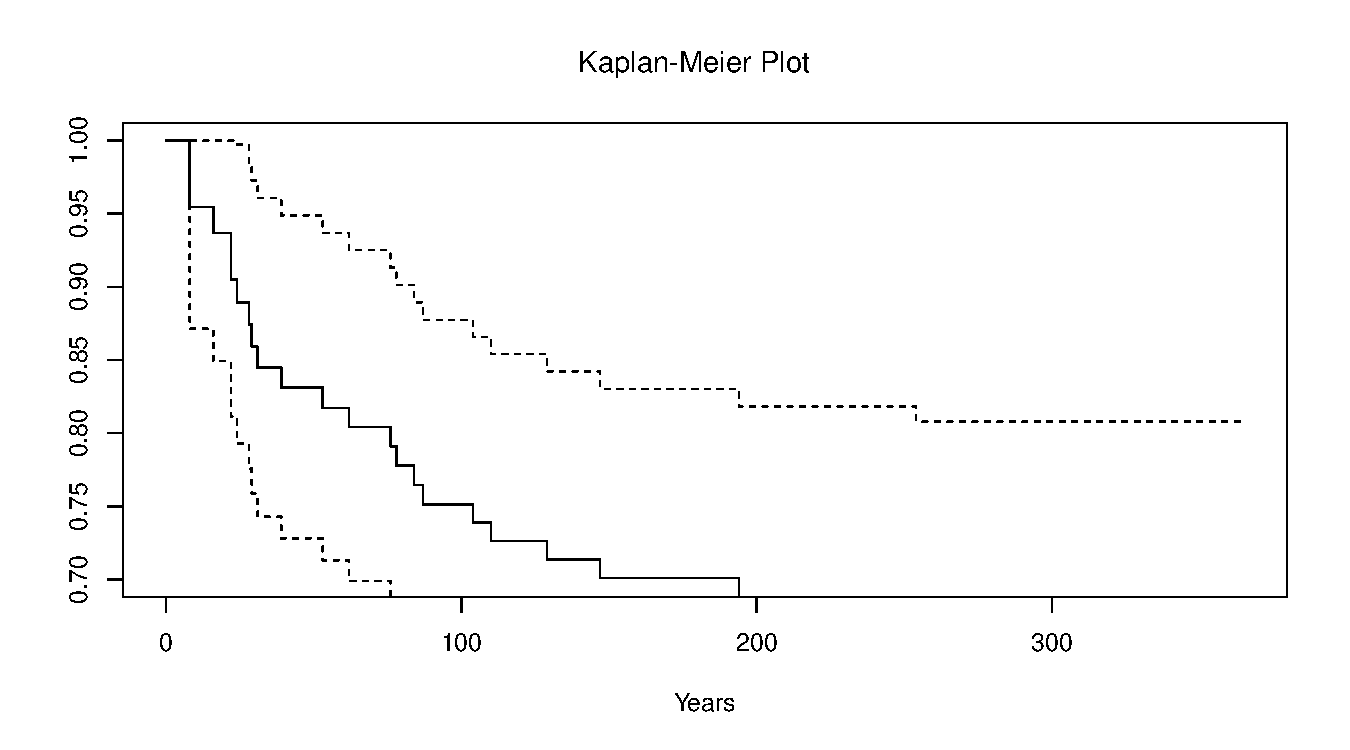
\includegraphics[width=.75\textwidth]{km_infantsplot.pdf}
 \end{figure}

\end{document}
